% Appendix A

\chapter{Supplemental Information} % Main appendix title
\label{SuppInfo} % For referencing this appendix elsewhere, use \ref{AppendixA}
%\lhead{Supplemental Information} % This is for the header on each page - perhaps a shortened title
\fancyhead[RO,LE]{Appendix: Supplemental Information}
\fancyfoot{}
\fancyfoot[C]{\thepage}

%
%%%%%%%%%%%%%%%%%%%%%%%%%%%%%
\section{Supplemental material related to the MSL and NSL complexes}
%
\begin{figure}[h!]
\includegraphics[width=1\textwidth]{Figures/histoneMarkDistribution.png}
\begin{footnotesize}
\setlength{\abovecaptionskip}{0ex}
\caption[Distribution of histone marks along an active gene.]{\textsf{Schematic patterns of selected histone marks along an active gene. Histone modifications associated with active transcription are shown in green (methylation) and orange (acetylation), repressive histone marks are shown in blue. Active promoters are strongly labelled with H3K9ac and H3K4me3, surrounded by H3K4me2/1. Inactive genes are typically covered with H3K9me2/3, H4K20me3 and H3K27me3 that also peaks around the silenced promoters. The image is based on \citep{Barth2010}. Note that the signal of H4K16ac for dosage compensated genes in \textit{Drosophila} inreases towards the 3'-end.}}
\label{fig:histoneDistribution}
\end{footnotesize}
\end{figure}
%\subsection{Protein names}
%\begin{minipage}{\textwidth} % to avoid pagebreaks despite longtable environment
\begin{singlespacing}
\begin{small}
\setlength{\extrarowheight}{2pt}
%\vspace*{-2em}
\begin{longtable}[l]{>{\textsf\bgroup}p{5.5cm}<{\egroup} >{\textsf\bgroup}p{8.5cm}<{\egroup}} % defining the columns - these must match the widths defined for the mini pages down below!
\caption[Protein names of MSL- and NSL complex members in \textit{D.~melanogaster} and mammals.]{\textsf{Protein names of MSL- and NSL complex members in \textit{D.~melanogaster}, mouse and humans. Bold font indicates the name that I used throughout most of the manuscript unless noted otherwise. MSL = male-specific lethal, NSL = non-specific lethal}} \\ % the \\ is important!
%%%%%%%%%%%%%%%
% table title
\textbf{\textit{Drosophila}} & \textbf{Mammals}
\tabularnewline \hline
\endfirsthead 
%
\multicolumn{2}{c}%
{\tablename\ \thetable\ -- \textit{Continued from previous page}} \\[1ex]
\textbf{\textit{Drosophila}} & \textbf{Mammals}
\tabularnewline \toprule %\tabularnewline [1ex]
\endhead % Line(s) to appear at top of every page (except first)
\multicolumn{2}{r}{\textit{Continued on next page}} \\
\endfoot % Last line(s) to appear at the bottom of every page (except last)
\endlastfoot
%-----------------------
%%%%%%%%%%%%%%%
 \textbf{MOF} (males absent on first) & MYST1, hMOF, KAT8 (lysine acetyl transferase 8)
\tabularnewline \midrule
%--------------------------
\textbf{MSL1} & hMSL1
\tabularnewline \midrule
%--------------------------
\textbf{MSL2} & hMSL2, Msl2l1, Rnf184 (ring finger~184)
\tabularnewline \midrule
%--------------------------
\textbf{MSL3} & hMSL3, Msl31
\tabularnewline \midrule
%--------------------------
\textbf{MLE} (maleless) & DHX9 (aspartic-acid-glutamine-alanine-histidin (DEAH) box helicase~9)
\tabularnewline \midrule
%--------------------------
\textbf{NSL1}, waharan & hMSL1v1, Kansl1 (KAT8 regulatory NSL complex subunit~1)
\tabularnewline \midrule
%--------------------------
\textbf{NSL2}, dgt1~(dimmed gamma tubulin~1) & Kansl2 (KAT8 regulatory NSL complex subunit~2)
\tabularnewline \midrule
%--------------------------
\textbf{NSL3}, Rcd1~(reduction in cen\-tro\-somin dots) & Kansl3 (KAT8 regulatory NSL complex subunit~3)
\tabularnewline \midrule
%--------------------------
\textbf{MBD-R2} (methyl-binding domain protein) & PHF20~(plant homeo domain~(PHD) finger protein~20), GLEA2~(glioma-expressed antigen~2)
\tabularnewline \midrule
%--------------------------
\textbf{MCRS2}, dMCRS1, p78, Rcd5~(reduction in cen\-tro\-somin dots) & p78, MSP58~(microspherule protein~58)
\tabularnewline \midrule
%--------------------------
\textbf{WDS} (will die slowly) & WDR5 (tryptophan-aspartic acid~(WD) repeat domain~5)
%--------------------------
\tabularnewline \bottomrule
%-----------------------------
\label{tab:Names}
\end{longtable}
\end{small}
\end{singlespacing}
%\end{minipage}
%
%\subsection{Cancer-related observations}
\vspace*{-4em}
\begin{minipage}{\textwidth} % to avoid pagebreaks despite longtable environment
\begin{singlespacing}
\begin{small}
\setlength{\extrarowheight}{2pt}
\begin{longtable}[l]{>{\textsf\bgroup}p{2cm}<{\egroup} >{\textsf\bgroup}p{12.5cm}<{\egroup}} % defining the columns - these must match the widths defined for the mini pages down below!
\caption[Association of MSL and NSL complex members with human cancers.]{\textsf{Association of MSL and NSL complex members with human cancers. Note that I used the mammalian protein names, see \tref{tab:Names} for synonyms and \textit{Drosophila} names.}} \\ % the \\ is important!
%%%%%%%%%%%%%%%
% table title
\textbf{Protein} & \textbf{Observation}
\tabularnewline
%-----------------------
\toprule
 MYST1 & \begin{minipage}{12.5cm}
				\begin{itemize}[noitemsep,leftmargin=*]
					\item downregulated in colorectal, gastric, ovarian, hepatocellular, breast cancer and renal cell carcinoma \citep{Pfister2008,Giampieri2013,Liu2013,Wang2013,Cao2014,Zhang2014a}, loss of H4K16ac is a hallmark of numerous cancers \citep{Fraga2005}
					\item upregulated in human non-small-cell lung cancer \citep{Chen2014}
					\end{itemize}
				\end{minipage}
\tabularnewline \midrule
%--------------------------
MSL1 & single nucleotide polymorphism in \textit{MSL1} is associated with decreased risk of invasive serous ovarian cancer \citep{Peedicayil2010} 
\tabularnewline \midrule
%--------------------------
MSL3 & might enhance the proliferation of hematopoetic cells in acute myeloid leukemia \citep{Sinenko2010}
\tabularnewline \midrule
%--------------------------
PHF20 & \begin{minipage}{12.5cm}
\begin{itemize}[noitemsep, leftmargin=*]
\item auto-antibodies against PHF20 are positively correlated with the survival rate of neuroblastoma patients \citep{Fischer2001,Pallasch2005}
\item high expression in non-small-cell lung cancer \citep{Taniwaki2006}, genetic alteration of \textit{PHF20} are associated with its progression \citep{Bankovic2010}
\end{itemize}
\end{minipage}
\tabularnewline \midrule
%--------------------------
MCRS1 & \begin{minipage}{12.5cm}
					\begin{itemize}[noitemsep, leftmargin=*]
							\item oncogene with the potential for malignant cell transformation \cite{Okumura2005a,Hsu2012}
							\item upregulated in all investigated cancer types \citep{Shi2012,Wu2012,Lin2013,Zhong2013}
					\end{itemize}
				\end{minipage}
\tabularnewline \midrule
%--------------------------
WDR5 & implicated in the establishment and progression of leukemia due to its interaction with the methyl transferase MLL (mixed-lineage leukemia; reviewed by \citet{Wu2011a})
%--------------------------
\tabularnewline \bottomrule
%-----------------------------
\label{tab:cancer}
\end{longtable}
\end{small}
\end{singlespacing}
\end{minipage}

%
%\subsection{Enzymes within the complexes}
\begin{minipage}{\textwidth} % to avoid pagebreaks despite longtable environment
\begin{singlespacing}
\begin{small}
\setlength{\extrarowheight}{1.5pt}
\vspace*{-2em}
\begin{longtable}[l]{>{\textsf\bgroup}p{2cm}<{\egroup}>{\textsf\bgroup}p{2cm}<{\egroup} >{\textsf\bgroup}p{4cm}<{\egroup}} % defining the columns - these must match the widths defined for the mini pages down below!
\caption[Enzymes within the MSL and NSL complexes.]{\textsf{Enzymes within the MSL and NSL complexes.}} \\ % the \\ is important!
%%%%%%%%%%%%%%%
% table title
\textbf{Complex} & \textbf{Protein} & \textbf{Function}
\tabularnewline
%-----------------------
\toprule
MSL, NSL & MOF & histone acetyl transferase
\tabularnewline \midrule
\multirow{2}{*}{MSL} 	& MSL2 & E3 ubiquitin ligase \\
											& MLE & DNA and RNA helicase
\tabularnewline \midrule
NSL & NSL3 & putative hydrolase function 
\tabularnewline \bottomrule
%-----------------------------
\label{tab:enzymes}
\end{longtable}
\end{small}
\end{singlespacing}
\end{minipage}

%
%---------------------------------
%%% Figure NSL targets
\begin{figure}[tb]
	\begin{minipage}[c]{0.50\textwidth}
		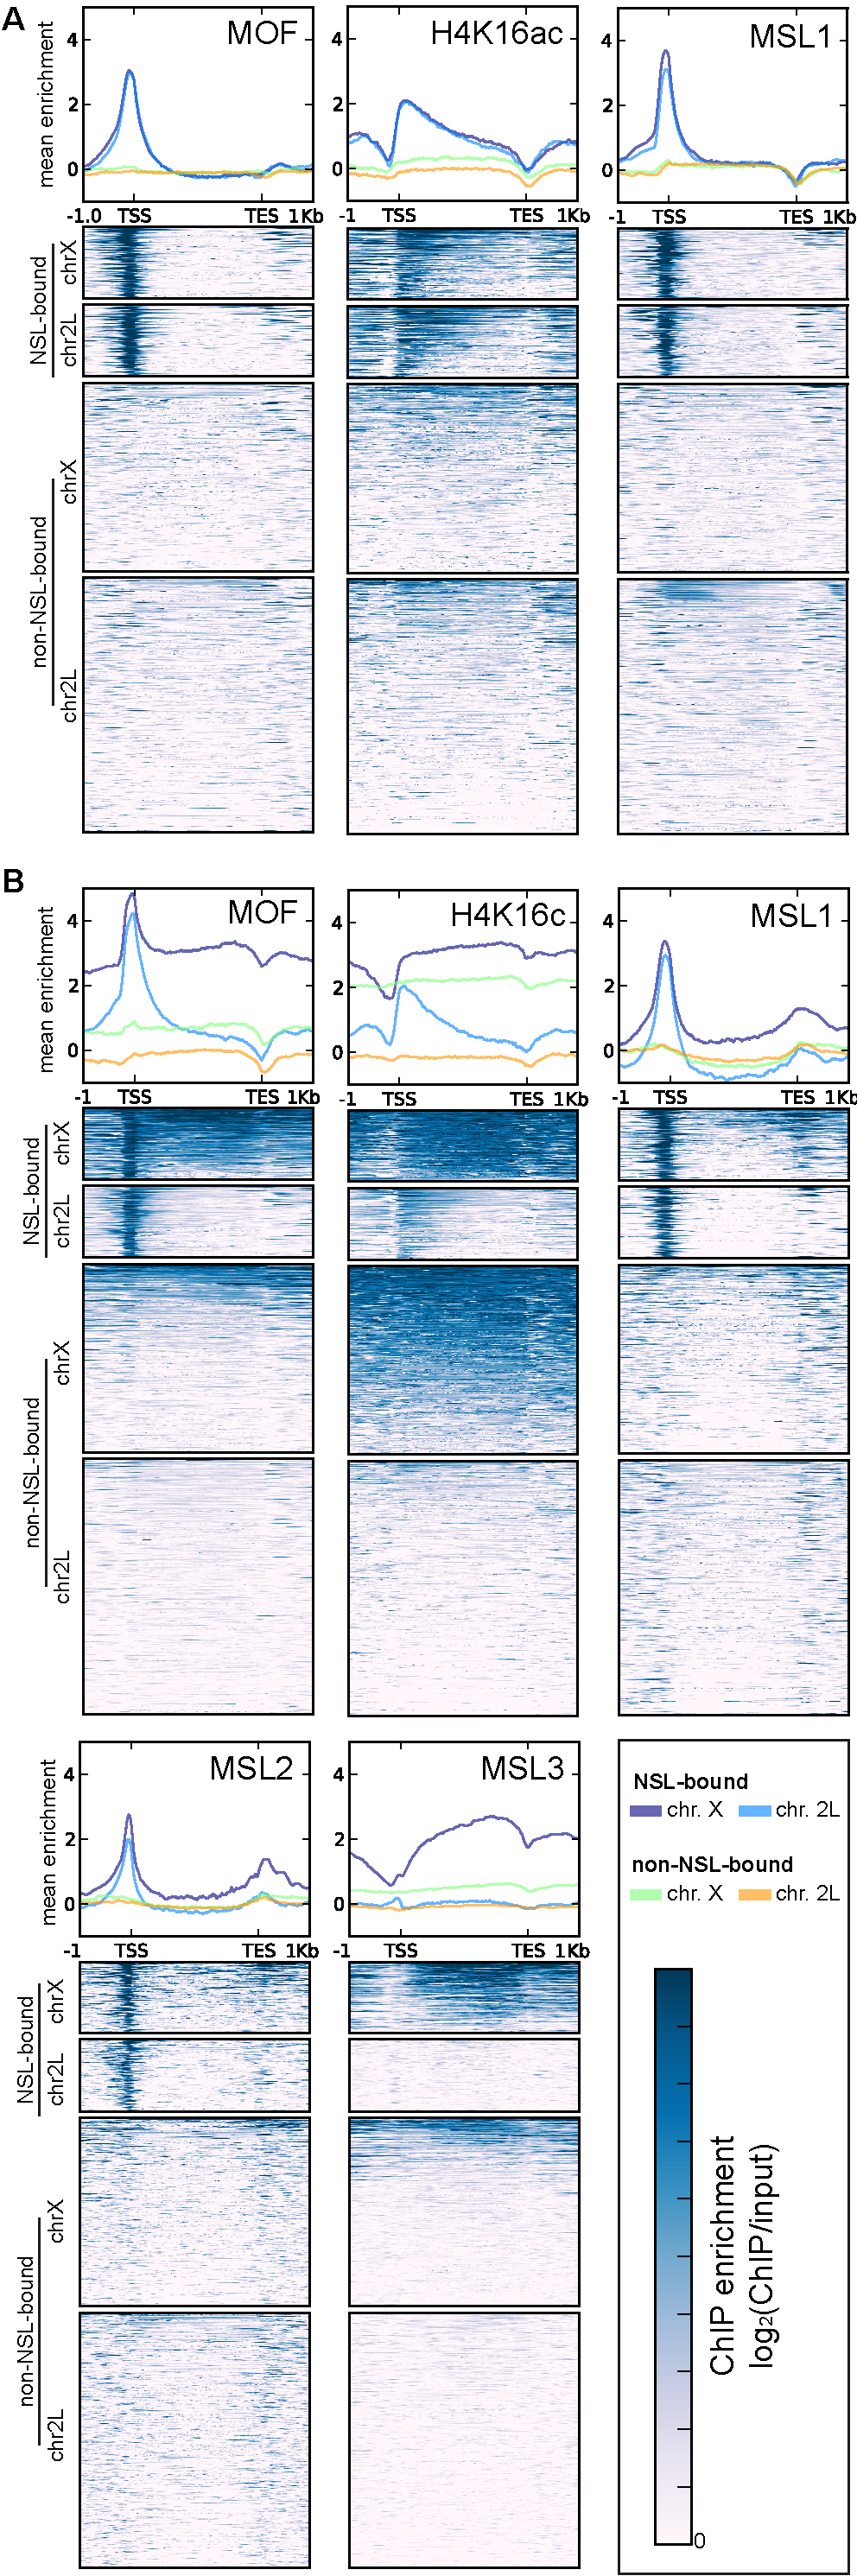
\includegraphics[width=\textwidth]{Figures/NSLtargetgenes_scissored.pdf}
	\end{minipage} \hfill
	%%%%%%%%%%
	\begin{minipage}[c]{0.4\textwidth}
		\begin{footnotesize}
			\caption[ChIP-seq signals of MSL complex members for NSL targets and NSL-non-bound genes in \textit{Drosophila}.]{\textsf{ChIP-seq signals of MSL complex members for NSL targets and NSL-non-bound genes in \textit{Drosophila}. All images were generated with \texttt{computeMatrix} and \texttt{heatmapper} from the deepTools suite \citep{Ramirez2014} using the scale-regions mode to scale gene bodies to 2~kb. See \tref{tab:ChIPseqSamplesDmel} and \ref{tab:Becker} for details about the ChIP-seq data sets.
\textbf{A)} There is no difference in the ChIP-seq signals of MOF, H4K16ac and MSL1 from female larva for autosomal (chromosome 2L, chr2L) and X-linked (chrX) genes, but there are almost exclusively strong enrichments for NSL targets.
\textbf{B)} In males, the signals of the MSL complex are visibly stronger for X-linked NSL targets, but only MSL3 and H4K16ac show significant enrichments for non-NSL-bound genes.}}
			\label{fig:NSLtargetgenes}
		\end{footnotesize}
	\end{minipage}
\end{figure}

\clearpage

%---------------------------------

%\vspace*{-2em}
%\begin{landscape}
\begin{minipage}{\textwidth}
\begin{singlespacing}
\begin{small}
\begin{sffamily}
\begin{longtable}[l]{>{\textsf\bgroup}p{3.8cm}<{\egroup} >{\raggedright\arraybackslash}p{2.7cm} >{\textsf\bgroup}p{7cm}<{\egroup}}
\caption[MOF-associated proteins in transcription activation.]{\textsf{MOF-associated proteins in transcription activation. Related to \fref{fig:functions}.}} \\ % the \\ is important! see http://tex.stackexchange.com/questions/103698/extra-alignment-tab-with-longtable
%%%%%%%%%%%%%%%
% table title
\textbf{Proteins} & \textbf{Function} & \textbf{Biological effect}
\tabularnewline \toprule
%\endfirsthead % indicates that the lines above appear as head of the table on the first page
%\multicolumn{3}{c}%
%{\tablename\ \thetable\ -- \textit{Continued from previous page}} \\ [2ex]
%\textbf{Proteins} & \textbf{Function} & \textbf{Biological effect}
%\tabularnewline \toprule \tabularnewline [1ex]
%\endhead % Line(s) to appear at top of every page (except first)
%\multicolumn{3}{r}{\textit{Continued on next page}} \\
%\endfoot % Last line(s) to appear at the bottom of every page (except last)
%\endlastfoot
%%%%%%%%%%%%%%%%%%%
%%% let's start the table content; each column (often) gets its own minipage which enables itemized lists etc.
%%%%%%%%%%%%%%%%%%%
%% first row
%-----------------------
%\\ \multicolumn{3}{c}{\textbf{\textsf{Gene expression}}}
%\\ [2ex] \hline \\ [1ex]
%------------------
\begin{minipage}[c]{3.8cm}
				\vskip 2pt
					MOF within the\\MSL complex \\
				(MSL1, MSL2,\\MSL3, MLE (roX))
				\vskip 2pt
			\end{minipage}
			& \begin{minipage}[c]{2.7cm}
					\raggedright acetylation of H4K16ac \citep{Akhtar2000,Taipale2005,Li2009} \\
			\end{minipage}
					& \begin{minipage}[c]{7cm}
					\vskip 2pt
									\begin{itemize}[noitemsep, leftmargin=*]
										\item opening of chromatin (reviewed by \citet{Preez2013})
										\item dosage compensation in male \textit{D.~melano\-gaster} that entails the upregulation of the entire X chromosome \citep{Conrad2011}
									\end{itemize}				
									\vskip 2pt
							\end{minipage}
%\\ [2ex] \hline \\ [1ex]
\tabularnewline \midrule
%-----------------------
\begin{minipage}[c]{3.8cm}
\vskip 2pt
					MOF within the\\NSL complex \\
				(NSL1, NSL2, NSL3,\\MCRS2, MBD-R2, WDS)
				\vskip 4pt
			\end{minipage}
			& \begin{minipage}[c]{2.7cm}
							\raggedright acetylation of H4K16 \citep{Li2009}, H4K5, H4K8 \citep{Cai2010}
			\end{minipage}
					& \begin{minipage}[c]{7cm} % 3rd column
									\begin{itemize}[noitemsep, leftmargin=*]
										\item opening of chromatin \citep{Preez2013}
										\item housekeeping gene regulation \citep{Feller2012, Lam2012}
									\end{itemize}				
							\end{minipage}
%\\ [2ex] \hline \\ [1ex]
\tabularnewline \midrule
%-----------------------
\begin{minipage}[c]{3.8cm}
					MSL2
			\end{minipage}
			& \begin{minipage}[c]{2.7cm}
			\vskip 2pt
					\raggedright ubiquitylation of H2BK34 \citep{Wu2011}
					\vskip 4pt
			\end{minipage}
					& \begin{minipage}[c]{7cm} % 3rd column
					\vskip 2pt
							implicated to stimulate methylation of H3K4 \citep{Wu2011} and transcription elongation \citep{Wu2014}
							\vskip 4pt
							\end{minipage}
\tabularnewline \midrule
%\\ [2ex] \hline \\ [1ex]
%-----------------------
\begin{minipage}[c]{3.8cm}
\vskip 2pt
					MCRS2
					\vskip 4pt
\end{minipage}
			& \begin{minipage}[c]{2.7cm}
			\vskip 2pt
					interaction partner
					\vskip 4pt
			\end{minipage}
					& \begin{minipage}[c]{7cm} % 3rd column
					\vskip 2pt
							facilitates Pol~II recruitment to target genes \citep{Andersen2010}
							\vskip 4pt
						\end{minipage}
%\\ [2ex] \hline\pagebreak
%-----------------------
%\multicolumn{3}{c}{\textbf{\textsf{Cell-cycle-associated processes}}}
%\\ [2ex] \hline \\ [1ex]
%-----------------------
%%%%%%%%%%%%%%%%%%%%%%%%%%
\tabularnewline \bottomrule
\label{tab:functions1}
\end{longtable}
\end{sffamily}
\end{small}
\end{singlespacing}
\end{minipage}

%%\vspace*{-2em}
\begin{minipage}{\textwidth}
\begin{singlespacing}
\begin{small}
\begin{sffamily}
\begin{longtable}[l]{>{\raggedright\arraybackslash}p{3cm} >{\raggedright\arraybackslash}p{11cm}}
\caption[MOF-associated proteins in cell-cycle-related processes.]{\textsf{MOF-associated proteins in cell-cycle-related processes. Related to \fref{fig:functions}}} \\ % the \\ is important! 
%%%%%%%%%%%%%%%
% table title
\textbf{Biological process} & \textbf{Observation} 
\tabularnewline \toprule
%==========================
\begin{minipage}[c]{3cm}
					G2/M checkpoint
			\end{minipage}
					& \begin{minipage}[c]{11cm} % 3rd column
					\vskip 4pt
							NSL1, NSL2, NSL3, MCRS2, MBD-R2 and WDS were identified as essential factors for G2/M checkpoint progression following DNA damage in \textit{D.~melano\-gaster} \citep{Kondo2011}
							\vskip 4pt
							\end{minipage}
\tabularnewline \midrule
%\\ [2ex] \hline \\ [1ex]
%-----------------------
\begin{minipage}[c]{3cm}
					mitotic spindle
			\end{minipage}
					& \begin{minipage}[c]{11cm} % 3rd column
					\vskip 4pt
							\begin{itemize}[noitemsep, leftmargin=*]
							\item NSL2 is needed for mitotic spindle assembly \citep{Goshima2007}
							\item MCRS1 stabilizes the mitotic spindle \citep{Meunier2011}
							\item WDS was identified in a screen for microtubule-associated proteins \cite{Hughes2008}
							\end{itemize}
							\vskip 2pt
							\end{minipage}
\tabularnewline \midrule
%------------------------
\begin{minipage}[c]{3cm}
					apoptosis
			\end{minipage}
					& \begin{minipage}[c]{11cm} % 3rd column
					\vskip 4pt
							\begin{itemize}[noitemsep, leftmargin=*]
							\item ubiquitylation of p53 by MSL2 leads to accumulation of p53 in the cytoplasm \citep{Kruse2009} which is necessary for apoptosis \cite{Muscolini2011}
							\item MOF acetylates p53 in the presence of NSL1 \citep{Li2009} which is necessary for apoptosis induction in cells with DNA damages \citep{Sykes2006, Sykes2009}
							\item human MBD-R2 (PHF20) stimulates expression of p53 and prevents its degradation via a direct interaction with methylated p53 \citep{Park2009, Cui2012}
							\end{itemize}
							\vskip 2pt
							\end{minipage}
\tabularnewline \midrule
%------------------------
\begin{minipage}[c]{3cm}
					DNA repair
			\end{minipage}
					& \begin{minipage}[c]{11cm} % 3rd column
					\vskip 4pt
							\begin{itemize}[noitemsep, leftmargin=*]
								\item MOF is generally required for repair of DNA double strand breaks and recruitment of 53BP1 and BRCA \cite{Sharma2010, Li2010}; its phosphorylated form is particularly important for biasing the cells towards homologous repair during S~phase by displacing 53BP1 from the site of the DNA damage \citep{Gupta2014}
								\item human MSL2 ubiquitylates 53BP1 \citep{Lai2013}
								\item human MSL1 interacts with 53BP1 that positively stimulates DNA damage repair \citep{Gironella2009}
							\end{itemize}
							\vskip 2pt
							\end{minipage}
%%%%%%%%%%%%%%%%%%%%%%%%%%
\tabularnewline \bottomrule
\label{tab:functions2}
\end{longtable}
\end{sffamily}
\end{small}
\end{singlespacing}
\end{minipage}
%
%%%%%%%%%%%%%%%%%%%%%%%%%%%%%%%%%
\section{Supplemental bioinformatics-related tables}
%
%\subsection{Bioinformatic tools and software}
%\begin{landscape}
\begin{singlespacing}
\begin{small}
%\setlength{\extrarowheight}{15pt} % this doesn't work to control the vertical space
\vspace*{-1em}
\begin{longtable}{>{\textsf\bgroup\raggedleft\arraybackslash}p{2.7cm}<{\egroup} >{\textsf\bgroup}p{4.5cm}<{\egroup} >{\textsf\bgroup}p{4.2cm}<{\egroup}>{\textsf\bgroup}p{2.3cm}<{\egroup}} % defining the columns - these must match the widths defined for the mini pages down below!
\caption[Bioinformatic tools used for analyses presented here.]{\textsf{Bioinformatic tools used for analyses presented here (alphabetical order; if available, I indicated the versions of the tools that I used). For explanations of the file formats mentioned here, please see the glossary within the supplement of \aref{SuppPub_deepTools}.}} \\ % the \\ is important! see http://tex.stackexchange.com/questions/103698/extra-alignment-tab-with-longtable
%%%%%%%%%%%%%%%
% table title
\textbf{Name} & \textbf{Application} & \textbf{Website} & \textbf{Reference}
\tabularnewline \hline
\endfirsthead % indicates that the lines above appear as head of the table on the first page
\multicolumn{4}{c}%
{\tablename\ \thetable\ -- \textit{Continued from previous page}} \\[1ex]
\textbf{Name} & \textbf{Application} & \textbf{Website} & \textbf{Reference}
\tabularnewline \toprule %\tabularnewline [1ex]
\endhead % Line(s) to appear at top of every page (except first)
\multicolumn{4}{r}{\textit{Continued on next page}} \\
\endfoot % Last line(s) to appear at the bottom of every page (except last)
\endlastfoot
%%%%%%%%%%%%%%%%%%%
%% first row
%-----------------------
\toprule %\\ [4ex]
 \begin{minipage}{2.7cm}
				\textbf{bedtools} \\
					(2.10. to 2.17)
				\end{minipage}
			&	 \begin{minipage}{4.5cm}
				working with genomic intervals, e.g. intersecting two files with different peak regions
			\end{minipage} 
			&  \begin{minipage}{4.2cm}
			\url{http://bedtools.readthedocs.org/en/latest/}
			\end{minipage} 
			&  \begin{minipage}{2.3cm}
					\raggedright \citet{Quinlan2010}
				\end{minipage} 
%\\ [4ex] \hline \\ [1ex]
\tabularnewline \midrule
%---------------------------
 \begin{minipage}{2.7cm}
				\textbf{bowtie} \\
					bowtie-1.0.0\\(Appendix \ref{SuppPub_NSL}),\\
					bowtie2-2.2.2\\(Appendix \ref{SuppPub_MSL}) %\\ [2ex]
			\end{minipage} 
			&  \begin{minipage}{4.5cm}
			alignment of reads to the reference genome
				\end{minipage} 
				&  \begin{minipage}{4.2cm}
				\url{http://bowtie-bio.sourceforge.net/index.shtml}
				\end{minipage} 
				&  \begin{minipage}{2.3cm}
				Langmead and\\
				Salzberg \citep{Langmead2012}
			\end{minipage} 
%\\ [4ex] \hline \\ [1ex]
\tabularnewline \midrule
%-----------------------
 \begin{minipage}{2.7cm}
				\textbf{ChIPEnrich}
			\end{minipage} 
			&  \begin{minipage}{4.5cm}
					gene ontology enrichments for target genes identified by ChIP-seq
			\end{minipage} 
			&  \begin{minipage}{4.2cm}
					\url{http://sartorlab.ccmb.med.umich.edu/chip-enrich}
			\end{minipage} 
			&  \begin{minipage}{2.3cm}
				\citet{Welch2014}
			\end{minipage} 
%\\ [4ex] \hline \\ [1ex]
\tabularnewline \midrule
%-----------------------------
 \begin{minipage}{2.7cm}
		\textbf{DAVID}
\end{minipage} 
			&  \begin{minipage}{4.5cm}
				gene identifier mapping and gene ontology term enrichment analyses
			\end{minipage} 
			&  \begin{minipage}{4.2cm}
				\url{http://david.abcc.ncifcrf.gov/}
			\end{minipage} 
				&  \begin{minipage}{2.3cm}
				\citet{Huang2009}
			\end{minipage} 
%\\ [4ex] \hline \\ [1ex]
\tabularnewline \midrule
%-----------------------------
 \begin{minipage}{2.7cm}
					\textbf{deepTools} \\
					(up to 1.5.7) %\\ [2ex]
			\end{minipage} 
			&  \begin{minipage}{4.5cm}
				quality controls of BAM files, normalizations, coverage file generation, visualizations with heatmaps and summary plots %\\ [2ex]
			\end{minipage} 
			&  \begin{minipage}{4.2cm}
				\url{http://deeptools.github.io/} %\\ [2ex]
			\end{minipage} 
				&  \begin{minipage}{2.3cm}
		\raggedright Ramirez, Dündar et al. \citep{Ramirez2014} %\\ [2ex]
			\end{minipage} 
%\\ [4ex] \hline \\ [1ex]
\tabularnewline \midrule
%-----------------------------
 \begin{minipage}{2.7cm}
					\textbf{DESeq}\\
					(1.10.1)
				\end{minipage} 
			&  \begin{minipage}{4.5cm}
				calculating normalized fold change values for Pol~II ChIP-seq data set \citep{EBIroutine}
			\end{minipage} 	
			&  \begin{minipage}{4.2cm}
				\url{http://www-huber.embl.de/users/anders/DESeq/}
			\end{minipage}
				& 
				\begin{minipage}{2.3cm}
		\citet{Anders2010}
			\end{minipage} 
%\\ [4ex] \hline \\ [1ex]
\tabularnewline \midrule
%---------------------------
 \begin{minipage}{2.7cm}
				\textbf{fastqc}
				\end{minipage}
			&  \begin{minipage}{4.5cm}
				quality control of FASTQ files
			\end{minipage} 
			&  \begin{minipage}{4.2cm}
				\url{http://www.bioinformatics.babraham.ac.uk/projects/fastqc/}
			\end{minipage} 
			&  not available
%\\ [4ex] \hline \\ [1ex]
\tabularnewline \midrule
%-----------------------------
 \begin{minipage}{2.7cm}
				\textbf{Galaxy} %%\\ [2ex]
				\end{minipage} 
			&  \begin{minipage}{4.5cm}
				vast collection of tools for manifold tasks including working with genomic intervals, joining of lists, motif search etc. %\\ [2ex]
			\end{minipage} 
			&  \begin{minipage}{4.2cm}
				in-house installation %%\\ [2ex]
			\end{minipage} 
					&  \begin{minipage}{2.3cm}
		\citet{Goecks2010} %%\\ [2ex]
			\end{minipage} 
%\\ [4ex] \hline \\ [1ex]
\tabularnewline \midrule
%-----------------------------
 \begin{minipage}{2.7cm}
					\textbf{ggplot2}\\
					(0.9.3.1)
			\end{minipage} 
			&  \begin{minipage}{4.5cm}
				R package for highly customizable plots (e.g. boxplots, x-y plots, bar charts etc.)
			\end{minipage} 
			&  \begin{minipage}{4.2cm}
				\url{http://ggplot2.org/}
			\end{minipage} 
			&  \begin{minipage}{2.3cm}
		\citet{ggplot2}
			\end{minipage} 
%\\ [4ex] \hline \\ [1ex]
\tabularnewline \midrule
%-----------------------------
 \begin{minipage}{2.7cm}
					\textbf{GREAT}\\
					(2.0)
				\end{minipage} 
			&  \begin{minipage}{4.5cm}
				web-based tool for target gene prediction
			\end{minipage} 
			&  \begin{minipage}{4.2cm}
				\url{http://bejerano.stanford.edu/great/public/html/}
			\end{minipage} 
				&  \begin{minipage}{2.3cm}
		\citet{McLean2010}
			\end{minipage} 
%\\ [4ex] \hline \\ [1ex]
\tabularnewline \midrule
%----------------------------
 \begin{minipage}{2.7cm}
					\textbf{Integrative\\Genomics\\Viewer}\\
					(up to 2.3.32) %\\ [2ex]
			\end{minipage} 
			& 	\begin{minipage}{4.5cm}
				genome browser for visualization of BAM, BED, bigWig and bedGraph files %\\ [2ex]
			\end{minipage} 
			&  \begin{minipage}{4.2cm}
				\url{http://www.broadinstitute.org/igv/} %\\ [2ex]
			\end{minipage} 
				&  \begin{minipage}{2.3cm}
		\citet{Thorvaldsdottir2013} %\\ [2ex]
			\end{minipage} 
%\\ [4ex] \hline \\ [1ex]
\tabularnewline \midrule
%-----------------------------
 \begin{minipage}{2.7cm}
					\textbf{liftover}\\
					(2013)
			\end{minipage} 
			&  \begin{minipage}{4.5cm}
				conversion of sequence coordinates from mm8 assembly to mm9
			\end{minipage} 
			&  \begin{minipage}{4.2cm}
				\url{https://genome.ucsc.edu/cgi-bin/hgLiftOver}
			\end{minipage} 
				&  not available
%\\ [4ex] \hline \\ [1ex]
\tabularnewline \midrule
%-----------------------------
 \begin{minipage}{2.7cm}
				\textbf{MACS}\\
					(1.4.2)
				\end{minipage}
			&	 \begin{minipage}{4.5cm}
				identification of significantly enriched ChIP-seq regions
			\end{minipage} 
			&  \begin{minipage}{4.2cm}
				\url{http://liulab.dfci.harvard.edu/MACS/}
			\end{minipage} 
				&  \begin{minipage}{2.3cm}
		\citet{Zhang2008}
			\end{minipage} 
%\\ [4ex] \hline \\ [1ex]
\tabularnewline \midrule
%-----------------------------
 \begin{minipage}{2.7cm}
				\textbf{MEME}\\
					(4.9.0)
				\end{minipage} 
			&  \begin{minipage}{4.5cm}
				\textit{de novo} DNA motif identification
			\end{minipage}
			&  \begin{minipage}{4.2cm}
				\url{http://meme.nbcr.net/meme/}
			\end{minipage} 
					&  \begin{minipage}{2.3cm}
		\raggedright  \citet{Bailey1994, Machanick2011}
			\end{minipage} 
%\\ [4ex] \hline \\ [1ex]
\tabularnewline \midrule
%-----------------------------
\begin{minipage}{2.7cm}
				\textbf{PeakSplitter}\\
					(1.0)
				\end{minipage} 
			&  \begin{minipage}{4.5cm}
				splitting peak regions predicted by MACS into separate regions based on local minima detection
			\end{minipage} 
			&  \begin{minipage}{4.2cm}
				\url{http://www.ebi.ac.uk/research/bertone/software}
			\end{minipage} 
			&  \begin{minipage}{2.3cm}
		\citet{Salmon2010}
			\end{minipage} 
%\\ [4ex] \hline \\ [1ex]
\tabularnewline \midrule
%-----------------------------
 \begin{minipage}{2.7cm}
					\textbf{samtools}\\
					(0.1.19)
			\end{minipage} 
			&	 \begin{minipage}{4.5cm}
				SAM and BAM file handling (indexing, number of mapped/unmapped and uniquely reads etc.)
			\end{minipage} 
			&  \begin{minipage}{4.2cm}
				\url{http://samtools.sourceforge.net/}
			\end{minipage} 
				&  \begin{minipage}{2.3cm}
		\citet{Li2009}
			\end{minipage} 
%\\ [4ex] \hline \\ [1ex]
\tabularnewline \midrule
%-----------------------------
 \begin{minipage}{2.7cm}
					\textbf{TRAP}\\
					(Annotate v3.04)
				\end{minipage} 
			&  \begin{minipage}{4.5cm}
				transcription factor binding affinity calculation
			\end{minipage} 
			&  \begin{minipage}{4.2cm}
				\url{http://trap.molgen.mpg.de/PASTAA.htm}
			\end{minipage} 
				&  \begin{minipage}{2.3cm}
		\citet{Roider2007}
			\end{minipage} 
%\\ [4ex] \hline \\ [1ex]
\tabularnewline \midrule
%-----------------------------
 \begin{minipage}{2.7cm}
				\textbf{UCSC tools} \\
					(2013)
				\end{minipage} 
			&  \begin{minipage}{4.5cm}
				format conversion (bedGraph to bigWig)
			\end{minipage} 
			&  \begin{minipage}{4.2cm}
				\url{http://www.broadinstitute.org/igv/}
			\end{minipage} 
					&  \begin{minipage}{2.3cm}
		\citet{Kent2010}
			\end{minipage} 
%\\ [4ex] \hline \\ [1ex]
\tabularnewline \midrule
%-----------------------------
 \begin{minipage}{2.7cm}
				\textbf{Venny}\\
					(2007)
				\end{minipage} 
			& 	\begin{minipage}{4.5cm}
				generation of Venn diagrams
			\end{minipage} 
			&  \begin{minipage}{4.2cm}
				\url{http://bioinfogp.cnb.csic.es/tools/venny/}
			\end{minipage} 
			&  not available
%\\ [4ex] \hline \\ [1ex]
\tabularnewline \bottomrule
%-----------------------------
\label{tab:tools}
\end{longtable}
\end{small}
\end{singlespacing}
%\end{landscape}

% Quality Metrics of ChIP-seq experiments
\input{Tables/Table_QScores}
%\subsection{Peak calling}
\begin{landscape}
\begin{singlespacing}
\begin{small}
\begin{longtable}{>{\textsf\bgroup}p{3.5cm}<{\egroup} >{\textsf\bgroup}p{4cm}<{\egroup} >{\textsf\bgroup}p{8cm}<{\egroup}>{\textsf\bgroup}p{6.5cm}<{\egroup}} % defining the columns - these must match the widths defined for the mini pages down below!
\caption[Peak calling strategies adjusted for the different sample characteristics.]{\textsf{Peak calling strategies adjusted for the different ChIP-seq sample characteristics.}} \\ % the \\ is important! 
%%%%%%%%%%%%%%%
% table title
\textbf{ChIP-seq sample} & \textbf{Issues} & \textbf{Strategy} &  % 
\tabularnewline \hline
\endfirsthead % indicates that the lines above appear as head of the table on the first page
\multicolumn{4}{c} 
{\tablename\ \thetable\ -- \textit{Continued from previous page}} \\
\textbf{ChIP-seq samples} & \textbf{Issues} & \textbf{Strategy} &  % 
\tabularnewline \toprule \tabularnewline [1ex]
\endhead % Line(s) to appear at top of every page (except first)
\hline \multicolumn{4}{r}{\textit{Continued on next page}} \\ %
\endfoot % Last line(s) to appear at the bottom of every page (except last)
\endlastfoot
%%%%%%%%%%%%%%%%%%%
%%% let's start the table content; each column (often) gets its own minipage which enables itemized lists etc.
%%%%%%%%%%%%%%%%%%%
%% first row
%-----------------------
\toprule
\begin{minipage}[c]{3.5cm}
NSL1, NSL3,\\MCRS2, MBD-R2 in\\\textit{D.~melanogaster}
\end{minipage}
			& \begin{minipage}[c]{4cm}
			peak regions often contained more than one local maximum due to the gene-dense nature of the \textit{Drosophila} genome
			\end{minipage}
				& \begin{minipage}[c]{8cm}
				\begin{enumerate}[noitemsep, leftmargin=*]
					\item peak calling with MACS 1.4.2 with default parameters \citep{Feng2012}
					\item peaks with FDR $\leq$ 5\%
					\item identification of smaller \textsl{subpeaks} with PeakSplitter \citep{Salmon2010}
				\end{enumerate}
				\end{minipage}
					& \begin{minipage}[c]{6.5cm}
					\parbox[c]{1em}{
						\includegraphics[width=6.5cm,trim=2 2 2 2,clip]{Figures/PeakCalling_Dmel}}
				\end{minipage} 
%\\ [2ex]  \hline \\ [1ex]
\tabularnewline \midrule
%-----------------------
\begin{minipage}[c]{3.5cm}
Pol~II in\\\textit{D.~melanogaster} cells\\(depleted of NSL1 or NSL3)
\end{minipage}
	& \begin{minipage}[c]{4cm}
	the mixed signal of Pol~II (localized, TF-like enrichments around TSS, broad, shallow enrichments along gene bodies) was not well captured by MACS
		\end{minipage}
		& \begin{minipage}[c]{8cm}
\vskip 6pt
				\begin{enumerate}[noitemsep, leftmargin=*]
					\item a symmetric null distribution was fitted to regions with negative enrichments, i.e. where the input signal exceeded the ChIP signal \citep{EBIroutine} (black line)
					\item genomic bins that deviated from the expectation (compare the blue with the black line) were determined as significantly enriched (threshold: q-value $\leq$ 0.05) \\ [2ex]
				\end{enumerate}
\vskip 4pt
			\end{minipage}
				& \begin{minipage}[c]{6.5cm}
						\parbox[c]{1em}{
						\includegraphics[width=6.5cm,trim=4 4 4 4,clip]{Figures/PeakCalling_PolII}}
					\end{minipage}
%\\ [2ex] \hline \\ [1ex]
\tabularnewline \midrule
%-----------------------
\begin{minipage}[c]{3.5cm}
MOF, MSL1, MSL2,\\NSL3, MCRS1 in\\ mouse ESCs and NPCs
\end{minipage}
	& \begin{minipage}[c]{4cm}
	non-optimal signal-noise ratios, GC bias
		\end{minipage}
		& \begin{minipage}[c]{8cm}
\vskip 6pt
				\begin{enumerate}[noitemsep, leftmargin=*]
                    \item in ESCs: adjustment of the GC bias in the input sample to match each ChIP-seq sample's GC bias
					\item peak calling with MACS 1.4.2 with default parameters \citep{Feng2012} for each ChIP-seq replicate (blue boxes) and the merged file (red box)
					\item only peaks that were present in both replicates and met the FDR threshold of $\leq$ 1\% were used \\ [2ex]
				\end{enumerate}
\vskip 4pt
			\end{minipage}
				& \begin{minipage}[c]{6.5cm}
\vskip 6pt
						\parbox[c]{1em}{
						\includegraphics[width=5.5cm,trim=4 4 4 4,clip]{Figures/PeakCalling_Mm}} 
\vskip 4pt
					\end{minipage}
%\\ [2ex] \hline \\ [1ex]
%-----------------------
\tabularnewline \bottomrule
\label{tab:peakCallingStrategies}
\end{longtable}
\end{small}
\end{singlespacing}
\end{landscape}
%
\subsection{Datasets}
\label{Datasets}
All analyses were enriched by the integration of previously published, publicly available high-throughput sequencing data and annotation.\\
%
\begin{minipage}{\textwidth} % to avoid pagebreaks despite longtable environment
\begin{singlespacing}
\begin{small}
\setlength{\extrarowheight}{2pt}
%\vspace*{-2em}
\begin{longtable}[l]{>{\textsf\bgroup}p{2cm}<{\egroup} >{\textsf\bgroup}p{6cm}<{\egroup} >{\textsf\bgroup}p{6cm}<{\egroup}} % defining the columns - these must match the widths defined for the mini pages down below!
\caption[Publicly available data bases that were used.]{\textsf{Publicly available data bases that were used.}} \\ % the \\ is important!
%%%%%%%%%%%%%%%
% table title
\textbf{Name} & \textbf{Application} & \textbf{Website}
\tabularnewline
%-----------------------
\toprule
 ArrayExpress & up- and download of high-throughput sequencing data (only raw read files) & \url{http://www.ebi.ac.uk/arrayexpress/} 
\tabularnewline \midrule
%--------------------------
 BioMart & mapping of gene and transcripts between different annotations for genome version mm9, e.g. Ensembl and RefSeq; download of non-protein-coding transcripts & \url{http://may2012.archive.ensembl.org/biomart/martview/} 
\tabularnewline \midrule
%--------------------------
 FlyBase & download of gene lists and genome sequence & \url{http://flybase.org/} 
\tabularnewline \midrule
%--------------------------
GEO & up- and download of high-throughput sequencing data (raw and processed data) & \url{http://www.ncbi.nlm.nih.gov/geo/} 
\tabularnewline \midrule
%--------------------------
HomoloGene & list of orthologous genes in \textit{Drosophila}, mice and humans & \url{http://www.ncbi.nlm.nih.gov/homologene} 
\tabularnewline \midrule
%--------------------------
\raggedright UCSC Table Browser & RefSeq gene lists, mappability tracks, GC content tracks, mouse DNase hypersensitivity tracks & \url{https://genome.ucsc.edu/}
%--------------------------
\tabularnewline \bottomrule
%-----------------------------
\label{tab:DB}
\end{longtable}
\end{small}
\end{singlespacing}
\end{minipage}

%
All samples generated by members of the Akhtar lab were uploaded to public repositories. Accession numbers starting with G indicate the GEO database, accession numbers starting with E indicate ArrayExpress (see \tref{tab:DB}). The DNA read numbers are based on filtered reads. Read and accession numbers refer to all available replicates of each experiment.
%
\subsubsection{\textit{Drosophila} datasets}
%
The subsequently listed data was used for Lam, Mühlpfordt, Vaquerizas et al. \citep{Lam2012} (\aref{SuppPub_NSL}) and Chlamydas et al.\\
\input{Tables/Table_DmelSamplesInHouse}
\clearpage
% TABLE: Public (non-in-house) data sets
\begin{singlespacing}
\begin{small}
\begin{sffamily}
\vspace*{-2em}
\begin{longtable}[l]{p{2.5cm}p{3.2cm}p{3cm}}
\caption[ChIP-chip modENCODE data sets from S2 cells.]{\textsf{ChIP-chip modENCODE data sets for which we downloaded the processed coverage files from GEO. All ChIP experiments were done in S2 cells.}} \\
%%%%%%%%%%%%%%%%%%%%%%%%%%%%%%%%%%%%%%%%%
% table title
\textbf{Sample} & \textbf{Downloaded data} & \textbf{Accession number} 
\tabularnewline \toprule
\endfirsthead % indicates that the lines above appear as head of the table on the first page
%
\multicolumn{3}{c}%
{\tablename\ \thetable\ -- \textit{Continued from previous page}} \\
\textbf{Sample} & \textbf{Downloaded data} & \textbf{Source} 
\tabularnewline \toprule \tabularnewline [1ex]
\endhead % Line(s) to appear at top of every page (except first)
%
\hline \multicolumn{3}{r}{\textit{Continued on next page}} \\
\endfoot % Last line(s) to appear at the bottom of every page (except last)
\endlastfoot
%%%%%%%%%%%%%%%%%%%%%%%%%%
%\tabularnewline \toprule
H3 & .bedgraph & GSM93208
\tabularnewline \midrule
%
H3K4me3 & .bedgraph & GSE20787
\tabularnewline \midrule
H3K36me3 & .bedgraph & GSE20785
\tabularnewline \midrule
H3K4me2 & .bedgraph & GSE23470
\tabularnewline \midrule
H4K5ac & .bedgraph & GSE20800
\tabularnewline \midrule
H3K9ac & .bedgraph & GSE20790
\tabularnewline \midrule
H4K8ac & .bedgraph & GSE20801
\tabularnewline \midrule
H3K9me3 & .bedgraph & GSE20794
\tabularnewline \midrule
H3K9me3 & .bedgraph & GSE20794
%%%%%%%%%%%%%%%%%%%%%%%%%%%
\tabularnewline \bottomrule
\label{tab:modENCODE}
%%%%%%%%%%%%%%%%%%%%%%%%%%%%%%
\end{longtable}
%
\vspace{-2em}
%
\begin{minipage}{\textwidth}
\begin{longtable}[l]{p{2.5cm}p{3.2cm}p{3cm}}
\caption[Publicly available ChIP-seq data of MSL complex members in \textit{Drosophila}.]{\textsf{ChIP-seq data of MSL complex members, downloaded and processed by Fidel Ramírez and used for \fref{fig:profiles}.}} \\
%%%%%%%%%%%%%%%%%%%%%%%%%%%%%%%%%%%%%%%%%
% table title
\textbf{Sample} & \textbf{Accession number} 
\tabularnewline \toprule
MSL2 & GSE37864
\tabularnewline \midrule
MSL3 & GSE37864
\tabularnewline \midrule
MLE & SRX111555
\tabularnewline \bottomrule
\label{tab:Becker}
%%%%%%%%%%%%%%%%%%%%%%%%%%%%%%
\end{longtable}
\end{minipage}
\end{sffamily}
\end{small}
\end{singlespacing}


%%%%%%%%%%%%%%%%%%%%%%%%%%%%%%%%%%%%
\subsubsection{Mouse datasets}
The following data was used for Chelmicki, Dündar et al.\citep{Chelmicki2014} (\aref{SuppPub_MSL}). MSL1 and input samples were also used for Chlamydas et al. (\aref{SuppPub_MSL1}). \\
\input{Tables/Table_MmSamplesInHouse}
\input{Tables/Table_RNASeqSamples}
\begin{singlespacing}
\begin{small}
\begin{sffamily}
\vspace*{-2em}
\begin{longtable}[l]{p{4.3cm}p{3.2cm}p{6.5cm}}
%%%%%%%%%%%%%%%%%%%%%%%%%%%
\caption[Publicly available mouse data sets and annotation.]{\textsf{Publicly available mouse data sets and annotation that were used for Chelmicki, Dündar et al.\citep{Chelmicki2014} (\aref{SuppPub_MSL})}} \\
%%%%%%%%%%%%%%%%%%%%%%%%%%%
\textbf{Sample} & \textbf{Downloaded data} & \textbf{Source} 
\tabularnewline \toprule
\endfirsthead % indicates that the lines above appear as head of the table on the first page
%
\multicolumn{3}{c}%
{\tablename\ \thetable\ -- \textit{Continued from previous page}} \\[1ex]
\textbf{Sample} & \textbf{Downloaded data} & \textbf{Source} 
%\tabularnewline \toprule %\tabularnewline [1ex]
\endhead % Line(s) to appear at top of every page (except first)
%
\hline \multicolumn{3}{r}{\textit{Continued on next page}} \\
\endfoot % Last line(s) to appear at the bottom of every page (except last)
\endlastfoot
%%%%%%%%%%%%%%%%%%%%%%%%%%%
Enhancers defined by histone marks & .bed-file of peaks & supplement of \citet{Creyghton2010}
\tabularnewline \midrule
%-----------------------
Super/typical enhancers & .bed-file of regions & supplement of \citet{Whyte2013}
\tabularnewline \midrule
%-----------------------
RNA Pol II ChIP-seq (mESC) & .wig-file of signal & GSM632040
\tabularnewline \midrule
%-----------------------
RNA Pol II ChIP-seq (mNPC) & .wig-file of signal & GSM632050
\tabularnewline \midrule
%-----------------------
p300 ChIP-seq (mESC) & .wig-file of signal & GSM723018
\tabularnewline \midrule
%-----------------------
H3K4me1 ChIP-seq (mESC) & .wig-file of signal & GSM723016
\tabularnewline \midrule
%-----------------------
H3K27ac ChIP-seq (mESC) & FASTQ file & GSM1005503
\tabularnewline \midrule
%-----------------------
CpG methylation (mESC) & .tsv-file of counts & GSE30202
\tabularnewline \midrule
%-----------------------
CpG methylation (mNPC) & .tsv-file of counts & GSE30202
\tabularnewline \midrule
%-----------------------
\raggedright DNase hypersensitivity (mESC) & .wig-file of signal & \raggedright from the UCSC Genome~Browser: wgEncodeUwDnaseEscj7S129ME0SigRep1
\tabularnewline \bottomrule
%-----------------------
\label{tab:PublicSamplesMM}
\end{longtable} 
\end{sffamily}
\end{small}
\end{singlespacing}

%%%%%%%%%%%%%%%%%%%%%%%%%%%%%
